\documentclass[border=10pt]{standalone}
\usepackage{tikz}
\usetikzlibrary{arrows.meta,positioning,calc,fit,backgrounds}
\usepackage{amsmath}
\usepackage[T1]{fontenc}
\usepackage{lmodern}

% Semantic palette: tensors (blue/lavender), learned transforms (pink),
% elementwise compute (yellow), collectives (green), gradients (peach).
\definecolor{ink}{HTML}{263238}
\definecolor{muted}{HTML}{5F6B73}
\definecolor{tensorfill}{HTML}{DCEAF7}
\definecolor{tensorline}{HTML}{3977A8}
\definecolor{weightfill}{HTML}{F6D9E2}
\definecolor{weightline}{HTML}{A44E70}
\definecolor{actfill}{HTML}{FFF0BE}
\definecolor{actline}{HTML}{A47713}
\definecolor{commfill}{HTML}{DDF0E4}
\definecolor{commline}{HTML}{3E8060}
\definecolor{gradfill}{HTML}{FBE3D2}
\definecolor{gradline}{HTML}{B76838}
\definecolor{panelbg}{HTML}{FAFBFC}
\definecolor{codebg}{HTML}{F1F3F4}
\definecolor{fwd}{HTML}{285F8F}
\definecolor{bwd}{HTML}{A34C2B}

\begin{document}
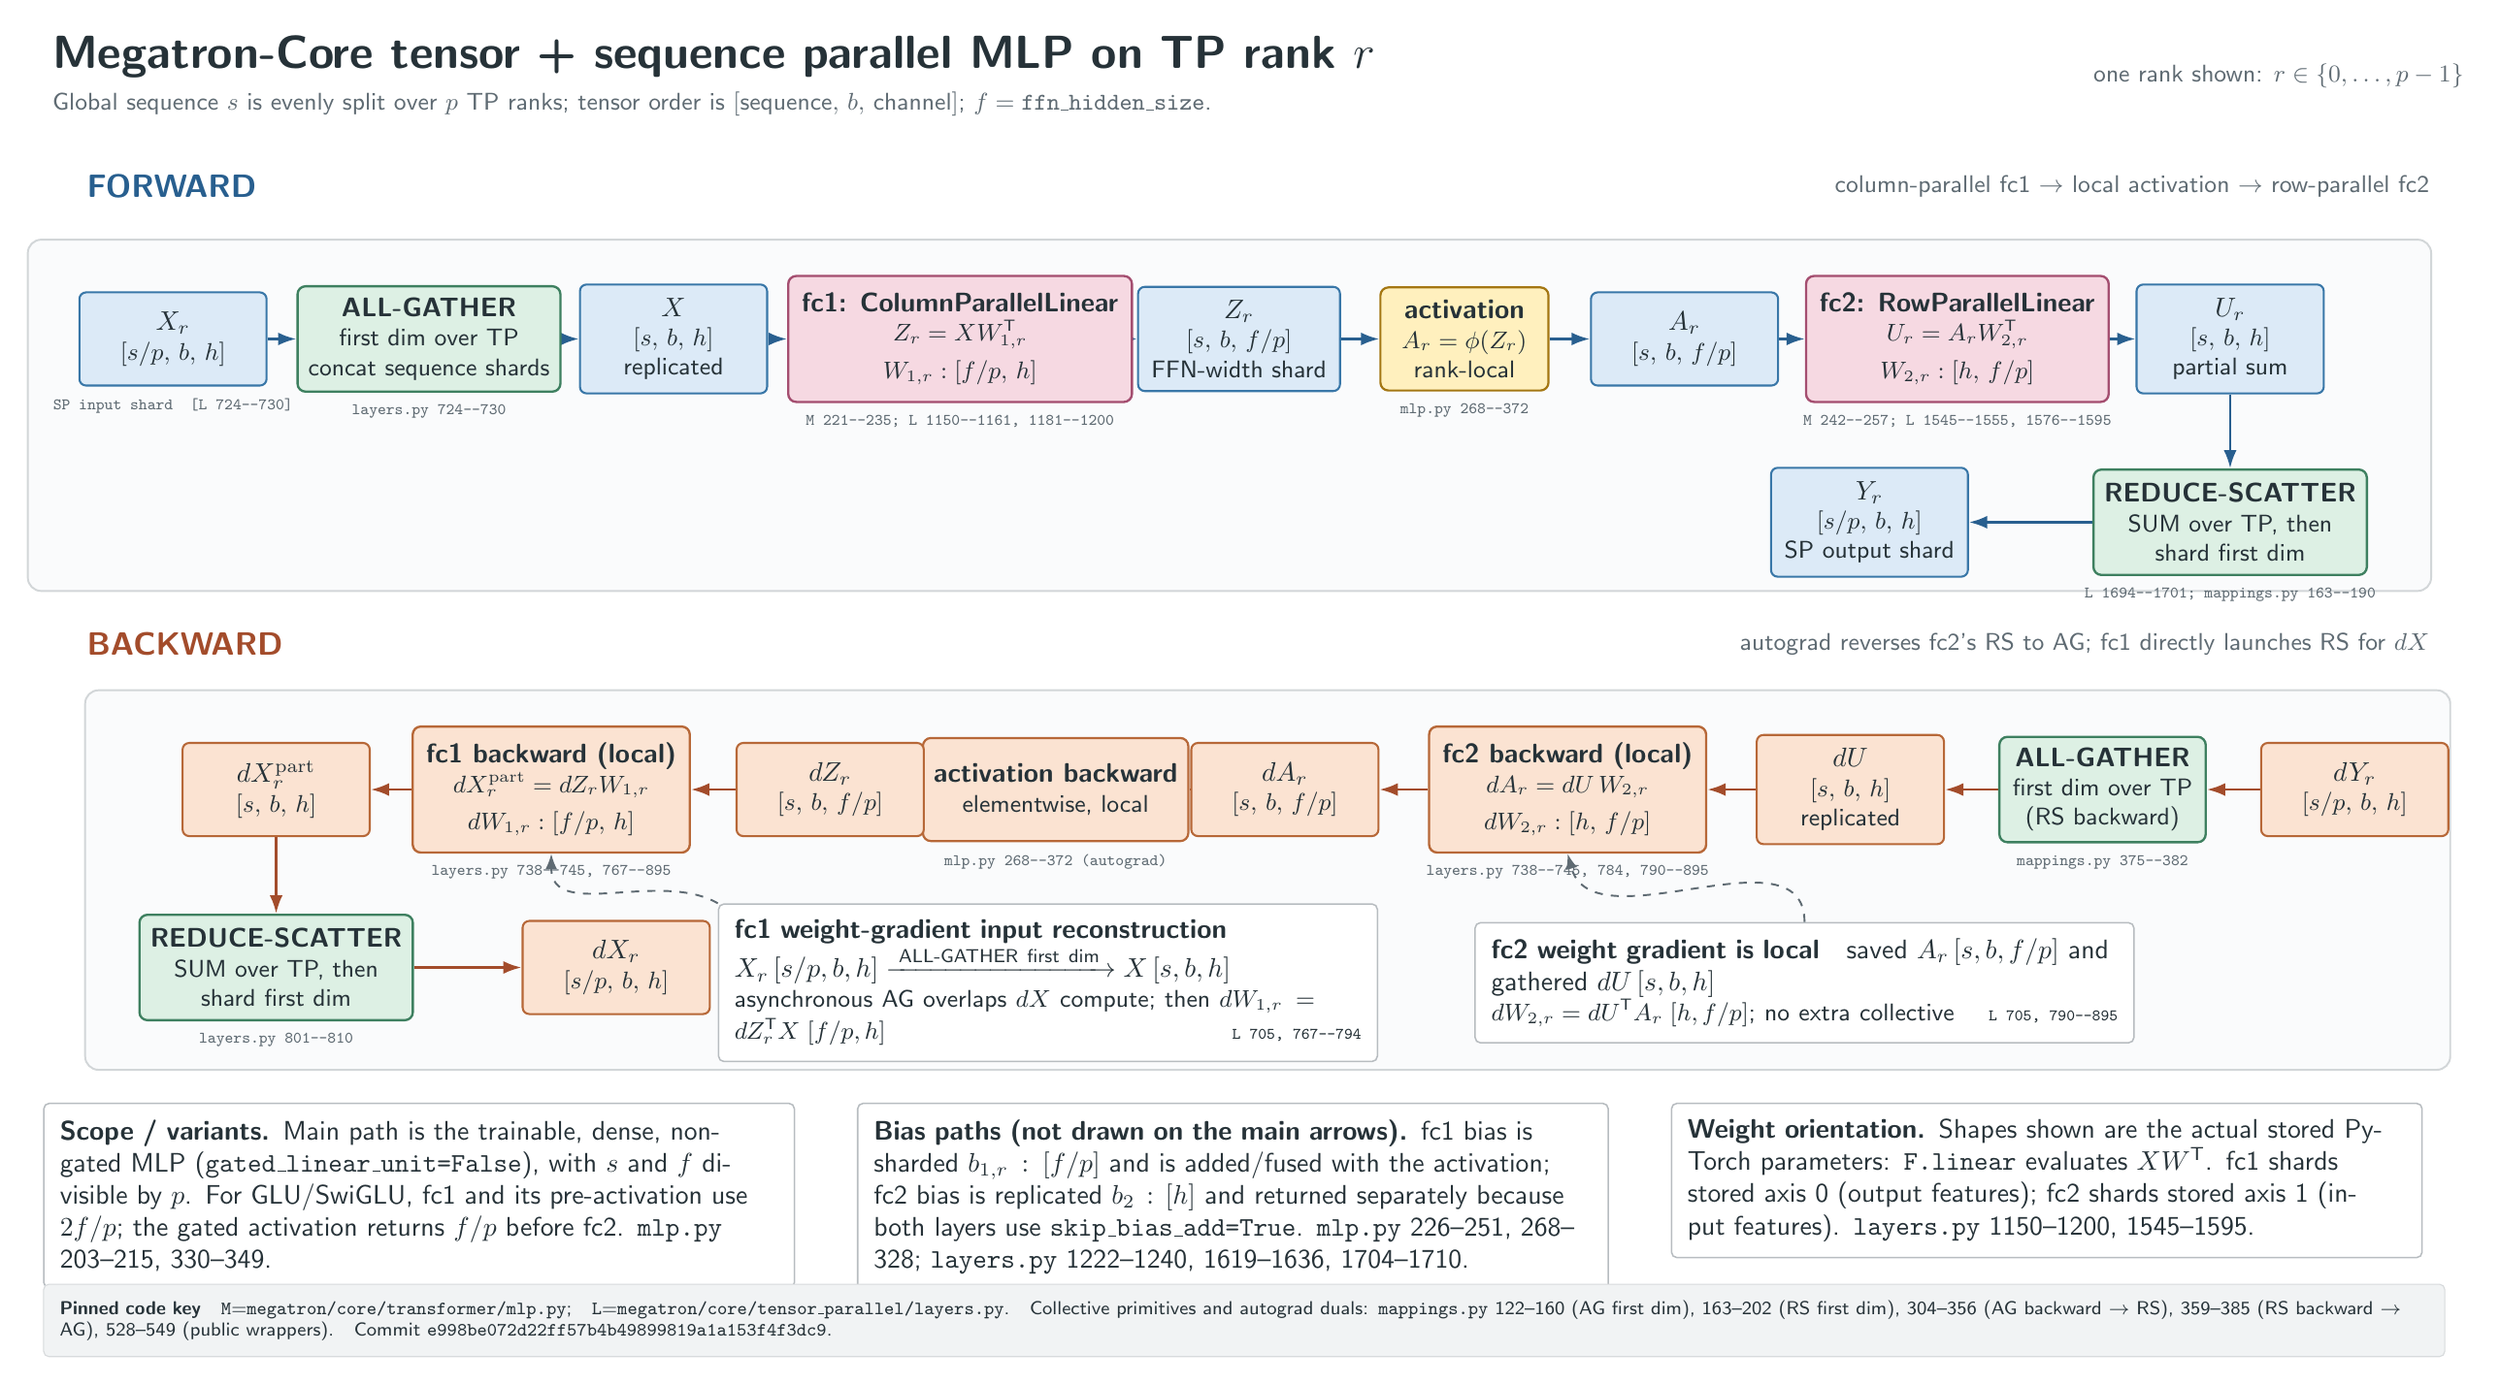
\begin{tikzpicture}[
  x=1cm,y=1cm,
  >=Latex,
  every node/.style={font=\sffamily, text=ink},
  tensor/.style={rounded corners=2.5pt, draw=tensorline, fill=tensorfill,
    line width=.75pt, minimum width=2.45cm, minimum height=1.22cm,
    align=center, inner sep=5pt},
  gradtensor/.style={rounded corners=2.5pt, draw=gradline, fill=gradfill,
    line width=.75pt, minimum width=2.45cm, minimum height=1.22cm,
    align=center, inner sep=5pt},
  linear/.style={rounded corners=3pt, draw=weightline, fill=weightfill,
    line width=.85pt, minimum width=3.2cm, minimum height=1.65cm,
    align=center, inner sep=5pt},
  activation/.style={rounded corners=3pt, draw=actline, fill=actfill,
    line width=.8pt, minimum width=2.2cm, minimum height=1.35cm,
    align=center, inner sep=4pt},
  collective/.style={rounded corners=3pt, draw=commline, fill=commfill,
    line width=.85pt, minimum width=2.7cm, minimum height=1.38cm,
    align=center, inner sep=4pt},
  paramgrad/.style={rounded corners=2.5pt, draw=weightline, fill=weightfill!65,
    line width=.7pt, minimum width=3.05cm, minimum height=1.12cm,
    align=center, inner sep=4pt},
  note/.style={rounded corners=2pt, draw=muted!45, fill=white,
    line width=.55pt, align=left, inner sep=6pt},
  code/.style={font=\ttfamily\fontsize{6.5}{7.5}\selectfont, text=muted},
  label/.style={font=\sffamily\small, text=muted, align=center},
  fwdarrow/.style={-{Latex[length=2.4mm,width=1.7mm]}, draw=fwd, line width=1.0pt},
  bwdarrow/.style={-{Latex[length=2.4mm,width=1.7mm]}, draw=bwd, line width=1.0pt},
  dataarrow/.style={-{Latex[length=2.0mm,width=1.5mm]}, draw=muted, line width=.7pt, dashed},
  panel/.style={rounded corners=5pt, draw=muted!28, fill=panelbg, line width=.7pt},
]

% ----------------------------------------------------------------------
% Title and notation
% ----------------------------------------------------------------------
\node[anchor=west, font=\sffamily\bfseries\LARGE] at (0,12.55)
  {Megatron-Core tensor + sequence parallel MLP on TP rank $r$};
\node[anchor=west, font=\sffamily\small, text=muted] at (0,11.92)
  {Global sequence $s$ is evenly split over $p$ TP ranks; tensor order is $[\text{sequence},\,b,\,\text{channel}]$; $f=\texttt{ffn\_hidden\_size}$.};
\node[anchor=east, font=\sffamily\small, text=muted] at (31.8,12.30)
  {one rank shown: $r\in\{0,\ldots,p-1\}$};

% Panel backgrounds are laid down before any arrows or nodes.
\begin{scope}[on background layer]
  \path[panel, rounded corners=5pt] (-.2,5.55) rectangle (31.25,10.15);
  \path[panel, rounded corners=5pt] (.55,-.72) rectangle (31.50,4.25);
\end{scope}

% ----------------------------------------------------------------------
% Forward panel
% ----------------------------------------------------------------------
\node[anchor=west, font=\sffamily\bfseries\large, text=fwd] at (.45,10.85)
  {FORWARD};
\node[anchor=east, font=\sffamily\small, text=muted] at (31.35,10.85)
  {column-parallel fc1 $\rightarrow$ local activation $\rightarrow$ row-parallel fc2};

\node[tensor] (xlocal) at (1.7,8.85)
  {$X_r$\\[-1pt]\small $[s/p,\,b,\,h]$};
\node[code, below=1pt of xlocal] {SP input shard\quad[L 724--730]};

\node[collective] (agf) at (5.05,8.85)
  {\textbf{ALL-GATHER}\\[-1pt]\small first dim over TP\\[-1pt]\small concat sequence shards};
\node[code, below=1pt of agf] {layers.py 724--730};

\node[tensor] (xfull) at (8.25,8.85)
  {$X$\\[-1pt]\small $[s,\,b,\,h]$\\[-1pt]\small replicated};

\node[linear] (fc1) at (12.0,8.85)
  {\textbf{fc1: ColumnParallelLinear}\\[-1pt]
   \small $Z_r=XW_{1,r}^{\mathsf T}$\\[2pt]
   \small $W_{1,r}: [f/p,\,h]$};
\node[code, below=1pt of fc1] {M 221--235; L 1150--1161, 1181--1200};

\node[tensor] (z) at (15.65,8.85)
  {$Z_r$\\[-1pt]\small $[s,\,b,\,f/p]$\\[-1pt]\small FFN-width shard};

\node[activation] (phi) at (18.60,8.85)
  {\textbf{activation}\\[-1pt]\small $A_r=\phi(Z_r)$\\[-1pt]\small rank-local};
\node[code, below=1pt of phi] {mlp.py 268--372};

\node[tensor] (a) at (21.48,8.85)
  {$A_r$\\[-1pt]\small $[s,\,b,\,f/p]$};

\node[linear] (fc2) at (25.05,8.85)
  {\textbf{fc2: RowParallelLinear}\\[-1pt]
   \small $U_r=A_rW_{2,r}^{\mathsf T}$\\[2pt]
   \small $W_{2,r}: [h,\,f/p]$};
\node[code, below=1pt of fc2] {M 242--257; L 1545--1555, 1576--1595};

\node[tensor] (u) at (28.62,8.85)
  {$U_r$\\[-1pt]\small $[s,\,b,\,h]$\\[-1pt]\small partial sum};

\node[collective, minimum width=3.15cm] (rsf) at (28.62,6.45)
  {\textbf{REDUCE-SCATTER}\\[-1pt]\small SUM over TP, then\\[-1pt]\small shard first dim};
\node[code, below=1pt of rsf] {L 1694--1701; mappings.py 163--190};

\node[tensor] (ylocal) at (23.9,6.45)
  {$Y_r$\\[-1pt]\small $[s/p,\,b,\,h]$\\[-1pt]\small SP output shard};

% Forward arrows behind the nodes.
\begin{scope}[on background layer]
  \draw[fwdarrow] (xlocal) -- (agf);
  \draw[fwdarrow] (agf) -- (xfull);
  \draw[fwdarrow] (xfull) -- (fc1);
  \draw[fwdarrow] (fc1) -- (z);
  \draw[fwdarrow] (z) -- (phi);
  \draw[fwdarrow] (phi) -- (a);
  \draw[fwdarrow] (a) -- (fc2);
  \draw[fwdarrow] (fc2) -- (u);
  \draw[fwdarrow] (u.south) -- (rsf.north);
  \draw[fwdarrow] (rsf) -- (ylocal);
\end{scope}

% ----------------------------------------------------------------------
% Backward panel
% ----------------------------------------------------------------------
\node[anchor=west, font=\sffamily\bfseries\large, text=bwd] at (.45,4.85)
  {BACKWARD};
\node[anchor=east, font=\sffamily\small, text=muted] at (31.35,4.85)
  {autograd reverses fc2's RS to AG; fc1 directly launches RS for $dX$};

\node[gradtensor] (dylocal) at (30.25,2.95)
  {$dY_r$\\[-1pt]\small $[s/p,\,b,\,h]$};

\node[collective] (agb) at (26.95,2.95)
  {\textbf{ALL-GATHER}\\[-1pt]\small first dim over TP\\[-1pt]\small (RS backward)};
\node[code, below=1pt of agb] {mappings.py 375--382};

\node[gradtensor] (du) at (23.65,2.95)
  {$dU$\\[-1pt]\small $[s,\,b,\,h]$\\[-1pt]\small replicated};

\node[linear, fill=gradfill, draw=gradline] (fc2b) at (19.95,2.95)
  {\textbf{fc2 backward (local)}\\[-1pt]
   \small $dA_r=dU\,W_{2,r}$\\[2pt]
   \small $dW_{2,r}: [h,\,f/p]$};
\node[code, below=1pt of fc2b] {layers.py 738--745, 784, 790--895};

\node[gradtensor] (da) at (16.25,2.95)
  {$dA_r$\\[-1pt]\small $[s,\,b,\,f/p]$};

\node[activation, fill=gradfill, draw=gradline] (phib) at (13.25,2.95)
  {\textbf{activation backward}\\[-1pt]\small elementwise, local};
\node[code, below=1pt of phib] {mlp.py 268--372 (autograd)};

\node[gradtensor] (dz) at (10.30,2.95)
  {$dZ_r$\\[-1pt]\small $[s,\,b,\,f/p]$};

\node[linear, fill=gradfill, draw=gradline] (fc1b) at (6.65,2.95)
  {\textbf{fc1 backward (local)}\\[-1pt]
   \small $dX_r^{\mathrm{part}}=dZ_rW_{1,r}$\\[2pt]
   \small $dW_{1,r}: [f/p,\,h]$};
\node[code, below=1pt of fc1b] {layers.py 738--745, 767--895};

\node[gradtensor] (dxpart) at (3.05,2.95)
  {$dX_r^{\mathrm{part}}$\\[-1pt]\small $[s,\,b,\,h]$};

\node[collective] (rsb) at (3.05,.62)
  {\textbf{REDUCE-SCATTER}\\[-1pt]\small SUM over TP, then\\[-1pt]\small shard first dim};
\node[code, below=1pt of rsb] {layers.py 801--810};

\node[gradtensor] (dxlocal) at (7.50,.62)
  {$dX_r$\\[-1pt]\small $[s/p,\,b,\,h]$};

% Backward main arrows.
\begin{scope}[on background layer]
  \draw[bwdarrow] (dylocal) -- (agb);
  \draw[bwdarrow] (agb) -- (du);
  \draw[bwdarrow] (du) -- (fc2b);
  \draw[bwdarrow] (fc2b) -- (da);
  \draw[bwdarrow] (da) -- (phib);
  \draw[bwdarrow] (phib) -- (dz);
  \draw[bwdarrow] (dz) -- (fc1b);
  \draw[bwdarrow] (fc1b) -- (dxpart);
  \draw[bwdarrow] (dxpart.south) -- (rsb.north);
  \draw[bwdarrow] (rsb) -- (dxlocal);
\end{scope}

% Saved-input / parameter-gradient lane. This is a second backward AG, used
% only to reconstruct fc1's full-sequence activation for its wgrad GEMM.
\node[note, text width=8.2cm] (savedlane) at (13.15,.42) {
  \textbf{fc1 weight-gradient input reconstruction}\quad
  $X_r\,[s/p,b,h]\xrightarrow{\;\text{ALL-GATHER first dim}\;}X\,[s,b,h]$\\[-1pt]
  \small asynchronous AG overlaps $dX$ compute; then
  $dW_{1,r}=dZ_r^{\mathsf T}X\;[f/p,h]$
  \hfill\raisebox{0pt}[0pt][0pt]{\ttfamily\fontsize{6.5}{7.5}\selectfont L 705, 767--794}
};
\node[note, text width=8.2cm] (savedfc2) at (23.05,.42) {
  \textbf{fc2 weight gradient is local}\quad
  saved $A_r\,[s,b,f/p]$ and gathered $dU\,[s,b,h]$\\[-1pt]
  \small $dW_{2,r}=dU^{\mathsf T}A_r\;[h,f/p]$; no extra collective
  \hfill\raisebox{0pt}[0pt][0pt]{\ttfamily\fontsize{6.5}{7.5}\selectfont L 705, 790--895}
};
\draw[dataarrow] (savedlane.north west) to[out=150,in=-90] (fc1b.south);
\draw[dataarrow] (savedfc2.north) to[out=90,in=-75] (fc2b.south);

% ----------------------------------------------------------------------
% Assumptions, bias and code-key footer
% ----------------------------------------------------------------------
\node[note, anchor=north west, text width=9.4cm] (scope) at (0,-1.15) {
  \textbf{Scope / variants.} Main path is the trainable, dense, non-gated MLP
  ($\texttt{gated\_linear\_unit=False}$), with $s$ and $f$ divisible by $p$.
  For GLU/SwiGLU, fc1 and its pre-activation use $2f/p$; the gated activation
  returns $f/p$ before fc2. \texttt{mlp.py} 203--215, 330--349.
};
\node[note, anchor=north west, text width=9.4cm] (biasnote) at (10.65,-1.15) {
  \textbf{Bias paths (not drawn on the main arrows).} fc1 bias is sharded
  $b_{1,r}:[f/p]$ and is added/fused with the activation; fc2 bias is replicated
  $b_2:[h]$ and returned separately because both layers use
  \texttt{skip\_bias\_add=True}. \texttt{mlp.py} 226--251, 268--328;
  \texttt{layers.py} 1222--1240, 1619--1636, 1704--1710.
};
\node[note, anchor=north west, text width=9.4cm] (storage) at (21.30,-1.15) {
  \textbf{Weight orientation.} Shapes shown are the actual stored PyTorch
  parameters: \texttt{F.linear} evaluates $XW^{\mathsf T}$. fc1 shards stored
  axis 0 (output features); fc2 shards stored axis 1 (input features).
  \texttt{layers.py} 1150--1200, 1545--1595.
};

\node[anchor=north west, rounded corners=2pt, fill=codebg, draw=muted!25,
      text width=31.0cm, inner sep=6pt, font=\sffamily\scriptsize] at (0,-3.52) {
  \textbf{Pinned code key}\quad
  \texttt{M}=\texttt{megatron/core/transformer/mlp.py};\quad
  \texttt{L}=\texttt{megatron/core/tensor\_parallel/layers.py}.\quad
  Collective primitives and autograd duals:
  \texttt{mappings.py} 122--160 (AG first dim), 163--202 (RS first dim),
  304--356 (AG backward $\rightarrow$ RS), 359--385 (RS backward $\rightarrow$ AG),
  528--549 (public wrappers).\quad Commit \texttt{e998be072d22ff57b4b49899819a1a153f4f3dc9}.
};

\end{tikzpicture}
\end{document}
